%%%%%%%%%%%%%%%%%%%%%%%%%%%%%%%%%%%%%%%%%%%%%%%%%%%%%%%%%%%%%%%%%%%%%%
% How to use writeLaTeX: 
%
% You edit the source code here on the left, and the preview on the
% right shows you the result within a few seconds.
%
% Bookmark this page and share the URL with your co-authors. They can
% edit at the same time!
%
% You can upload figures, bibliographies, custom classes and
% styles using the files menu.
%
%%%%%%%%%%%%%%%%%%%%%%%%%%%%%%%%%%%%%%%%%%%%%%%%%%%%%%%%%%%%%%%%%%%%%%

\documentclass[12pt]{article}

\usepackage{sbc-template}

\usepackage{graphicx,url}

\usepackage{indentfirst}

%\usepackage[brazil]{babel}   
\usepackage[utf8]{inputenc}  
\

     
\sloppy

\title{Caracterização de bibliotecas de UI}

\author{Aylton B. de Almeida Junior\inst{1}, Lucca Romaniello Benjamin\inst{2}, Pedro Paulo Andrade\inst{3} }


\address{Engenharia de Software -- Pontifícia Universiade Catolica de Minas Gerais (PUC MG)\\
  Belo Horizonte -- MG -- Brazil
  \email{\{abajunior, lbenjamin, pedro.faria.1115474\}@sga.pucminas.br}
}

\begin{document} 

\maketitle

% \begin{abstract}
%   This meta-paper describes the style to be used in articles and short papers
%   for SBC conferences. For papers in English, you should add just an abstract
%   while for the papers in Portuguese, we also ask for an abstract in
%   Portuguese (``resumo''). In both cases, abstracts should not have more than
%   10 lines and must be in the first page of the paper.
% \end{abstract}
     
% \begin{resumo} 
%   Este meta-artigo descreve o estilo a ser usado na confecção de artigos e
%   resumos de artigos para publicação nos anais das conferências organizadas
%   pela SBC. É solicitada a escrita de resumo e abstract apenas para os artigos
%   escritos em português. Artigos em inglês deverão apresentar apenas abstract.
%   Nos dois casos, o autor deve tomar cuidado para que o resumo (e o abstract)
%   não ultrapassem 10 linhas cada, sendo que ambos devem estar na primeira
%   página do artigo.
% \end{resumo}

\section{Introdução}

"Nos últimos anos, tornar as coisas mais utilizáveis se tornou uma responsabilidade de quase todos. Agora, designers visuais e desenvolvedores costumam fazer coisas como design de interação (decidir o que acontece a seguir quando o usuário clica, toca ou desliza) e arquitetura de informações (descobrir como tudo deve ser organizado)". \cite{DONTMAKEMETHINK}.

Com base na citação de Steve Krug, percebemos que as interfaces visuais no mundo digital se tornam amplamente necessárias, especialmente para possiblitar que usuários completem das mais diversas tarefas em produtos digitais. Com o avanço da tecnologia e a crescente demanda por desenvolvimento de sistemas amigáveis aos usuários finais, bibliotecas que auxiliam a criação de interfaces de usuário se tornam cada vez mais frequentes no ramo do desenvolvimento.

Dessa forma, com o crescimento na utilização de frameworks web e de bibliotecas de UI \textit{(User Interface)}, surgem alguns questionamentos em relação à tais sistemas, como por exemplo:
\begin{enumerate}
  \item As bibliotecas mais populares são mais abertas a novos colaboradores?
  \item Bibliotecas baseadas nas linguagens mais populares possuem uma menor curva de aprendizado?
  \item As bibliotecas de UI se tornaram necessárias para os projetos atuais?
\end{enumerate}

Será realizado um experimento de medição de software para tentar responder os questionamentos apontados acima e, inicialmente, sua metodologia será descrita a seguir.

\section{Metodologia}

Para a realização da pesquisa será necessário recuperar dois grupos principais de dados, sendo o primeiro necessário para conseguir fazer a coleta do segundo. O primeiro grupo de dados é uma lista de 1000 repositórios de bibliotecas de componentes para construção de interfaces gráficas, utilizando de tópicos do Github para filtra-los. Já o segundo se trata de 1000 repositórios NodeJs, de forma que usaremos o arquivo \textit{package.json} do repositório para verificar se eles usam ou não alguma biblioteca de UI.

\subsection{Sobre a Questão 1}

A primeira métrica da questão 1 é a relação entre o número de \textit{Pull Requests} feitos por novos contribuidores pelo número total de \textit{PRs}. Para isso seram recuperados todos os \textit{Pull Requests} e seus autores, caso um autor possua apenas um \textit{PR} ele é um considerado novo autor. Já a segunda métrica é o tempo médio para aceitação de \textit{Pull Requests} feitos por novos contribuidores, esses que serão caracterizados da mesma forma que na métrica 1.

Ambas essas métricas são acessíveis por meio da API GraphQL do Github. Dessa forma um \textit{script} em Python será escrito, utilizando de cursores para ultrapassar o limite de 100 repositórios por \textit{request}. Esse código tem como objetivo gerar um arquivo csv contendo uma sumarização dos dados para analise posterior. 

\subsection{Sobre a Questão 2}

Primeiramente, assumimos que perguntas realizadas no site \textit{StackOverflow} associadas à tais linguagens possuem um percentual de respostas maior do que aquelas menos populares. Dessa forma, utilizando o \textit{Stack Exchange Data Explorer}, uma interface de consultas SQL na base dos sites pertencentes a essa stack (nesse caso, incluindo o \textit{StackOverflow}), será calculado o percentual de questões respondidas para as bibliotecas analisadas. 

Para complementar a formulação da resposta para a hipótese inicial, também será calculada a frequência de atualização de repositórios que utilizam as bibliotecas baseadas nas linguagens mais populares. Essa métrica se baseia na suposição que bibliotecas populares são atualizadas mais frequentemente e, dessa forma, se torna mais complexo manter o conhecimento relacionado àquela biblioteca atualizado. Para isso, será desenvolvido um programa em \textit{Python} que consulta a API GraphQL da empresa GitHub, esta que é provavelmente uma das principais plataformas de hospedagem de código fonte do mundo e que também armazena as principais bibliotecas \textit{open source} atualmente.


\subsection{Sobre a Questão 3}
Inicialmente será feita uma busca utilizando a API GraphQL do Github para encontrar todos os repositórios criados no ano de 2020.Em seguida um script desenvolvido em Python utilizando a biblioteca GitPy vai buscar os repositórios, checar se existe o arquivo "Package.json" e caso haja este arquivo, irá buscar a existência de algum nome dos repositórios encontrados o processo da Questão 1 e 2. 

Dessa forma será criado um filtro onde dividirá em duas frentes: repositórios que possuem bibliotecas de user interface e repositórios que não utilizam.

\subsection{Conclusão}
Sendo assim após toda a operação de recuperar os repositórios de bibliotecas relacionadas a UI do Github, buscar os repositórios criados em 2020 e filtrar todos estes dados entre os que utilizam alguma das bibliotecas e os que não utilizam de nenhuma biblioteca teremos dados suficientes para definir se o uso de bibliotecas UI se tornou uma característica relevante durante as criações de novos projetos.  

\begin{figure}[ht]
\centering
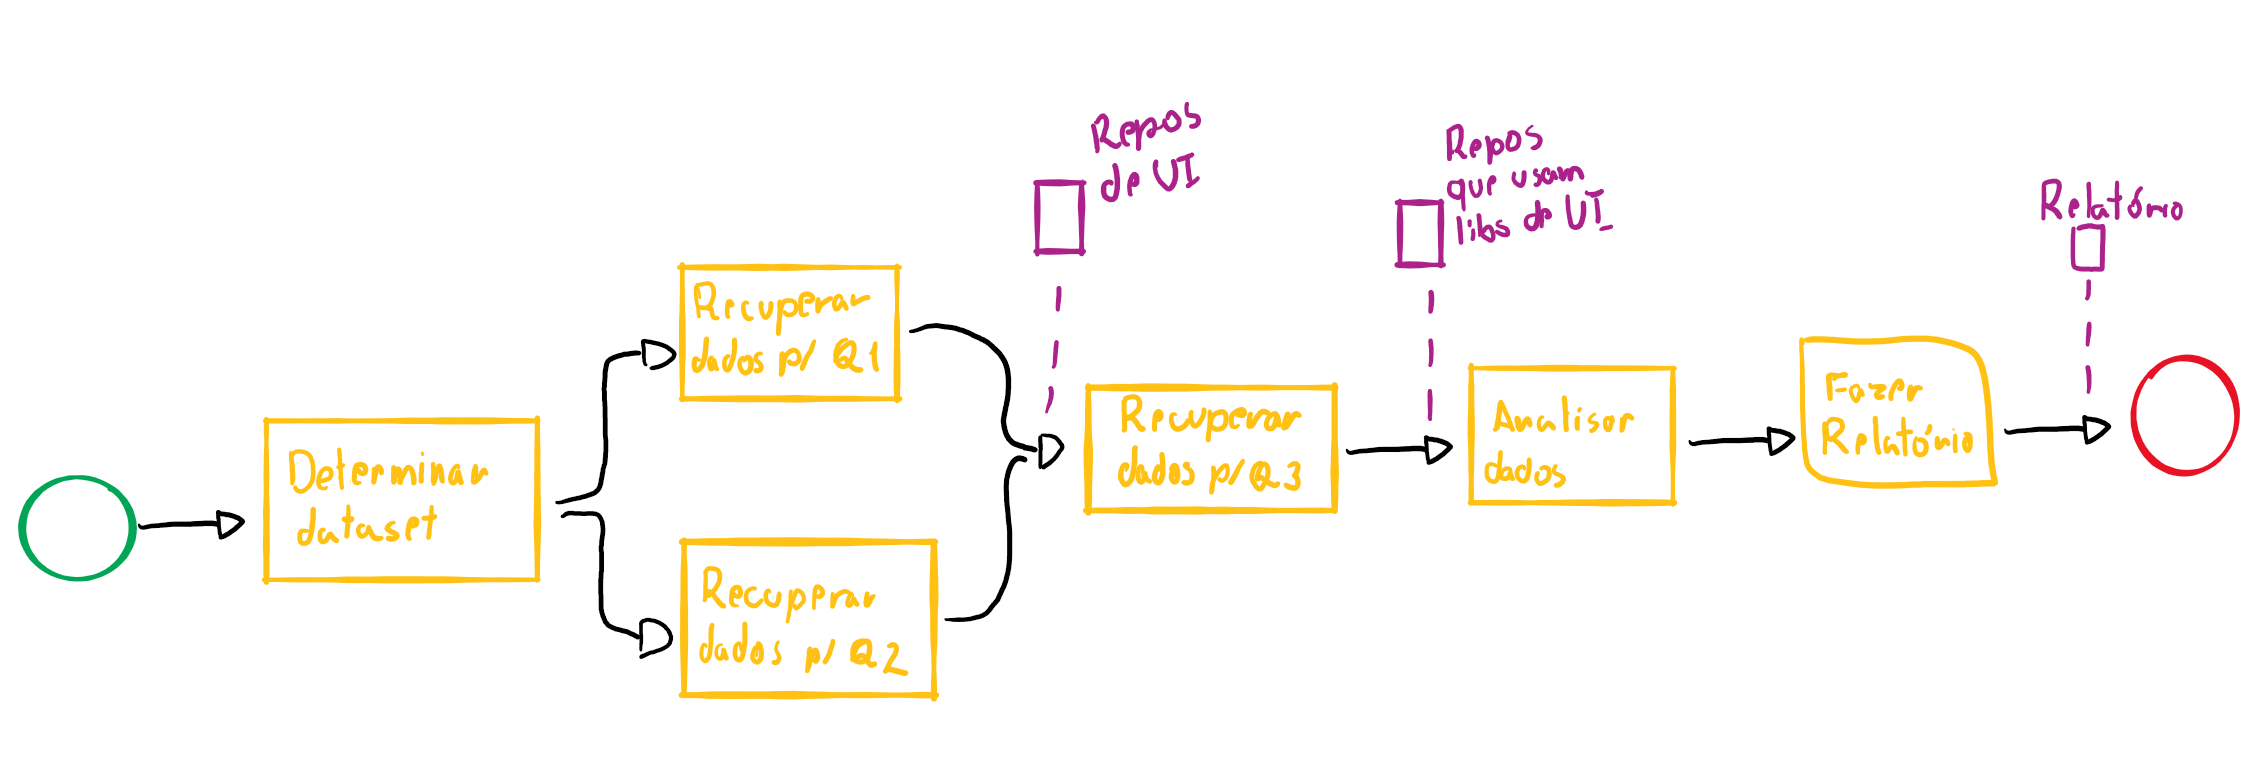
\includegraphics[width=1\textwidth]{assets/metodologia.png}
\caption{Imagem metodologia}
\label{fig:metdologia}
\end{figure}

\section{Referências}

Referências bibliográficas utilizadas pelo projeto: \cite{uiintegration:07}, \cite{componentengineering}, \cite{DESOLDA201746}, \cite{6606685}, \cite{materialui:21}, \cite{STATEOCTOVERSE}, \cite{EMPOWERINGUI}, \cite{DONTMAKEMETHINK}, \cite{OPENSOURCEUSABILITY}, \cite{OPENSOURCEADOPTION}, \cite{4196485}, \cite{779128}, \cite{6048455}, \cite{7490575}, \cite{9089992}

\bibliographystyle{sbc}
\bibliography{sbc-template}

\end{document}
